% Koko
\documentclass[black,normal,cn]{elegantnote}
\usepackage{array}
\newcolumntype{P}[1]{>{\centering\arraybackslash}p{#1}}
\newfontfamily\courier{Courier New}
\lstset{linewidth=1.1\textwidth,
	numbers=left,
	basicstyle=\small\courier,
	numberstyle=\tiny\courier,
	keywordstyle=\color{blue}\courier,
	commentstyle=\it\color[cmyk]{1,0,1,0}\courier, 
	stringstyle=\it\color[RGB]{128,0,0}\courier,
	frame=single,
	backgroundcolor=\color[RGB]{245,245,244},
	breaklines,
	extendedchars=false, 
	xleftmargin=2em,xrightmargin=2em, aboveskip=1em,
	tabsize=4, 
	showspaces=false
	basicstyle=\small\courier
}
\title{计算机网络技术实践报告}

\begin{document}
\begin{titlepage}
    \bfseries{2017211240}
    \vspace{4cm}
    \begin{center}
        \bfseries\huge{计算机网络技术实践}\\
        \vspace{0.5cm}
        \bfseries\huge{实验报告}
        \vspace{3cm}
        \begin{center}
          \large
          \linespread{2}
          \centering
          \renewcommand\arraystretch{1.6}
          \begin{tabular}{p{3cm}P{6cm}}
            \bfseries{实验名称:}       & VLAN 组网配置实验   \\ \cline{2-2}
            \bfseries{姓名:}           & 于海鑫   \\ \cline{2-2}
            \bfseries{学号:}           & 2017211240  \\ \cline{2-2}
            \bfseries{实验日期:}        & 2019.11.19 \\ \cline{2-2}
            \bfseries{报告日期:}        & 2019.12.07 \\ \cline{2-2}
          \end{tabular}
        \end{center}
      \end{center}
\end{titlepage}

\section{环境}
在本次实验中,我们使用的操作系统为 Windows 10 64 位专业版。网络平台为
CCNA 多用版虚拟实验室 By N.L.F.E v2.0 Base Dynamips 0.2.7。

\section{第一部分:VLAN 配置}

在这个一部分中,我们使用老师提供的拓扑文件进行配置,拓扑如下:

\includegraphics[width=0.9\textwidth]{ref1}

\subsection{实验过程}

\paragraph{环境准备}
首先我们将配置文件以及启动的 \texttt{cmd} 脚本放置到对应的位置,之后打开控制台开始准备实验。我们首先需要按例开启全部的 PC 机以及交换机,并打开 \texttt{telnet} 端口准备进行配置。配置流程如下:
\begin{lstlisting}
Reading configuration file...


Network successfully started

Dynagen management console for Dynamips

=> list
Name       Type       State      Server          Console
R1         7200       stopped    localhost:7200  3001
SW1        3640       stopped    localhost:7200  3003
SW2        3640       stopped    localhost:7200  3004
PC1        c2600      stopped    localhost:7200  3006
PC2        c2600      stopped    localhost:7200  3007
PC3        c2600      stopped    localhost:7200  3008
=> start SW1
Warining: Starting SW1 with no idle-pc value
100-C3600 'SW1' started
=> idlepc get SW1
Please wait while gathering statistics...
   1: 0x604f1484 [39]
   2: 0x604b99e8 [63]
   3: 0x604eaf94 [33]
*  4: 0x604eb174 [53]
   5: 0x604eb190 [36]
   6: 0x604eb200 [68]
*  7: 0x60423b48 [58]
   8: 0x604ebc1c [24]
   9: 0x604ebc58 [38]
  10: 0x60593c70 [37]
Potentially better idlepc values marked with "*"
Enter the number of the idlepc value to apply [1-10] or ENTER for no change: 7
Applied idlepc value 0x60423b48 to SW1

=> start SW2
Warining: Starting SW2 with no idle-pc value
100-C3600 'SW2' started
=> idlepc save SW1 db
idlepc value for image "unzip-c3640-js-mz.124-10.bin" written to the database
=> start PC1
Warining: Starting PC1 with no idle-pc value
100-C2600 'PC1' started
=> idlepc get PC1
Please wait while gathering statistics...
   1: 0x802c071c [25]
   2: 0x802c0730 [39]
*  3: 0x803553bc [52]
   4: 0x80357140 [50]
   5: 0x803772d0 [67]
   6: 0x80357960 [46]
   7: 0x80357acc [38]
Potentially better idlepc values marked with "*"
Enter the number of the idlepc value to apply [1-7] or ENTER for no change: 3
Applied idlepc value 0x803553bc to PC1

=> idlepc save PC1 db
idlepc value for image "unzip-c2600-i-mz.121-3.T.bin" written to the database
=> start PC2
100-C2600 'PC2' started
=> start PC3
100-C2600 'PC3' started
\end{lstlisting}

\paragraph{配置 IP}
我们将三台 PC 的 \texttt{F0/0} 端口配置为其对应 IP。下面记录了配置 PC1 的 IP 的过程,配置 PC2 和 PC3 的与之类似。
\begin{lstlisting}
Router>en
Router#conf
Configuring from terminal, memory, or network [terminal]?
Enter configuration commands, one per line.  End with CNTL/Z.
Router(config)#interface f0/0
Router(config-if)#ip add 1.1.1.1 255.255.255.0
Router(config-if)#no shutdown
Router(config-if)#exit
Router(config)#
00:11:58: %LINK-3-UPDOWN: Interface FastEthernet0/0, changed state to up
00:11:59: %LINEPROTO-5-UPDOWN: Line protocol on Interface FastEthernet0/0, changed state to up
\end{lstlisting}

\paragraph{配置 VLAN}
我们在 SW1 上配置 VLAN,配置流程如下:
\begin{lstlisting}
Router#en
Router#conf
Configuring from terminal, memory, or network [terminal]?
Enter configuration commands, one per line.  End with CNTL/Z.
Router(config)#exit
Router#
*Mar  1 00:16:59.515: %SYS-5-CONFIG_I: Configured from console by console
Router#
Router#
Router#vlan database
Router(vlan)#vlan 2
VLAN 2 added:
    Name: VLAN0002
Router(vlan)#vlan 3
VLAN 3 added:
    Name: VLAN0003
Router(vlan)#exit
APPLY completed.
Exiting....
Router#conf
Router#configure
Configuring from terminal, memory, or network [terminal]?
Enter configuration commands, one per line.  End with CNTL/Z.
Router(config)#inter
Router(config)#interface vlan 2
Router(config-if)#exit
Router(config)#interface vlan 3
Router(config-if)#exit
\end{lstlisting}

\paragraph{同一 VLAN 内互相 PING}
之后我们指定 SW1 的 \texttt{f1/11} 以及 \texttt{f1/12} 都位于 vlan 2 下,互相 \texttt{ping} 以查看是否可以联通。
SW 1 下面的配置如下:
\begin{lstlisting}
Router(config)#interface f1/11
Router(config-if)#swi
Router(config-if)#switchport access vlan 2
Router(config-if)#exit
Router(config)#
*Mar  1 00:18:12.275: %LINEPROTO-5-UPDOWN: Line protocol on Interface Vlan2, changed state to up
Router(config)#
Router(config)#interface f1/12
Router(config-if)#switchport access vlan 2
Router(config-if)#exit
\end{lstlisting}
PC 2 的结果如下:
\begin{lstlisting}
Router#
00:13:11: %SYS-5-CONFIG_I: Configured from console by console
Router#
Router#ping 1.1.1.1

Type escape sequence to abort.
Sending 5, 100-byte ICMP Echos to 1.1.1.1, timeout is 2 seconds:
.....
Success rate is 0 percent (0/5)
Router#ping 1.1.1.2

Type escape sequence to abort.
Sending 5, 100-byte ICMP Echos to 1.1.1.2, timeout is 2 seconds:
!!!!!
Success rate is 100 percent (5/5), round-trip min/avg/max = 1/3/4 ms
Router#ping 1.1.1.1

Type escape sequence to abort.
Sending 5, 100-byte ICMP Echos to 1.1.1.1, timeout is 2 seconds:
.!!!!
Success rate is 80 percent (4/5), round-trip min/avg/max = 4/12/20 ms
Router#ping 1.1.1.1

Type escape sequence to abort.
Sending 5, 100-byte ICMP Echos to 1.1.1.1, timeout is 2 seconds:
!!!!!
Success rate is 100 percent (5/5), round-trip min/avg/max = 1/5/8 ms
\end{lstlisting}
PC 1 的结果如下:
\begin{lstlisting}
Router#ping 1.1.1.2

Type escape sequence to abort.
Sending 5, 100-byte ICMP Echos to 1.1.1.2, timeout is 2 seconds:
!!!!!
Success rate is 100 percent (5/5), round-trip min/avg/max = 4/11/32 ms
\end{lstlisting}
可见可以互相 \texttt{ping} 通。

\paragraph{不同 VLAN 内互相 PING}
使用指令 \texttt{switchport access vlan 3} 将 SW1 的 \texttt{f
f1/12} 端口的 VLAN 设置为 3,之后进行互相 \texttt{ping}。结果如下:
PC1:
\begin{lstlisting}
Router#ping 1.1.1.2

Type escape sequence to abort.
Sending 5, 100-byte ICMP Echos to 1.1.1.2, timeout is 2 seconds:
.....
Success rate is 0 percent (0/5)
\end{lstlisting}
PC2:
\begin{lstlisting}
Router#ping 1.1.1.1

Type escape sequence to abort.
Sending 5, 100-byte ICMP Echos to 1.1.1.1, timeout is 2 seconds:
.....
Success rate is 0 percent (0/5)
\end{lstlisting}
可见在不同 VLAN 下的两个 PC 机无法直接通信。

\section{第二部分:交换机之间的 VLAN 配置}
\paragraph{直接添加 VLAN}
首先我们启动 PC3 并将之 IP 配置为 \texttt{1.1.1.3},然后启动 SW3,将 VLAN 2 写入到 SW2 的数据库内,SW2 的配置过程如下:
\begin{lstlisting}
Router>en
Router#vlan databae
                  ^
% Invalid input detected at '^' marker.

Router#vlan database
Router(vlan)#vlan 2
VLAN 2 added:
    Name: VLAN0002
Router(vlan)#exit
APPLY completed.
Exiting....
Router#conf
Configuring from terminal, memory, or network [terminal]?
Enter configuration commands, one per line.  End with CNTL/Z.
Router(config)#interface f1/11
Router(config-if)#switchport access vlan 2
Router(config-if)#exit
\end{lstlisting}
互PING结果如下:
PC1:
\begin{lstlisting}
Router#ping 1.1.1.3

Type escape sequence to abort.
Sending 5, 100-byte ICMP Echos to 1.1.1.3, timeout is 2 seconds:
.....
Success rate is 0 percent (0/5)
\end{lstlisting}
PC3:
\begin{lstlisting}
Router#ping 1.1.1.1

Type escape sequence to abort.
Sending 5, 100-byte ICMP Echos to 1.1.1.1, timeout is 2 seconds:
.....
Success rate is 0 percent (0/5)
\end{lstlisting}
此时不能联通,还需要更多的配置。

\paragraph{配置交换机之间的互连}
我们需要将交换机互连的端口设置为 \texttt{trunk} 模式。
SW 2 下面的配置如下:
\begin{lstlisting}
Router(config)#interface f1/1
Router(config-if)#Switchport mode Trunk
Router(config-if)#
*Mar  1 00:51:52.159: %DTP-5-TRUNKPORTON: Port Fa1/1 has become dot1q trunk
Router(config-if)#
Router(config-if)#Switchport trunk allowed vlan all
Router(config-if)#exit
\end{lstlisting}
PC 3 的结果如下:
\begin{lstlisting}
Type escape sequence to abort.
Sending 5, 100-byte ICMP Echos to 1.1.1.1, timeout is 2 seconds:
!!!!!
Success rate is 100 percent (5/5), round-trip min/avg/max = 1/4/12 ms
\end{lstlisting}
PC 1 的结果如下:
\begin{lstlisting}
Router#ping 1.1.1.3

Type escape sequence to abort.
Sending 5, 100-byte ICMP Echos to 1.1.1.3, timeout is 2 seconds:
!!!!!
Success rate is 100 percent (5/5), round-trip min/avg/max = 4/15/32 ms
\end{lstlisting}
可见可以互相 \texttt{ping} 通。

\section{不同 VLAN 互联}

我们使用的拓扑图如下:

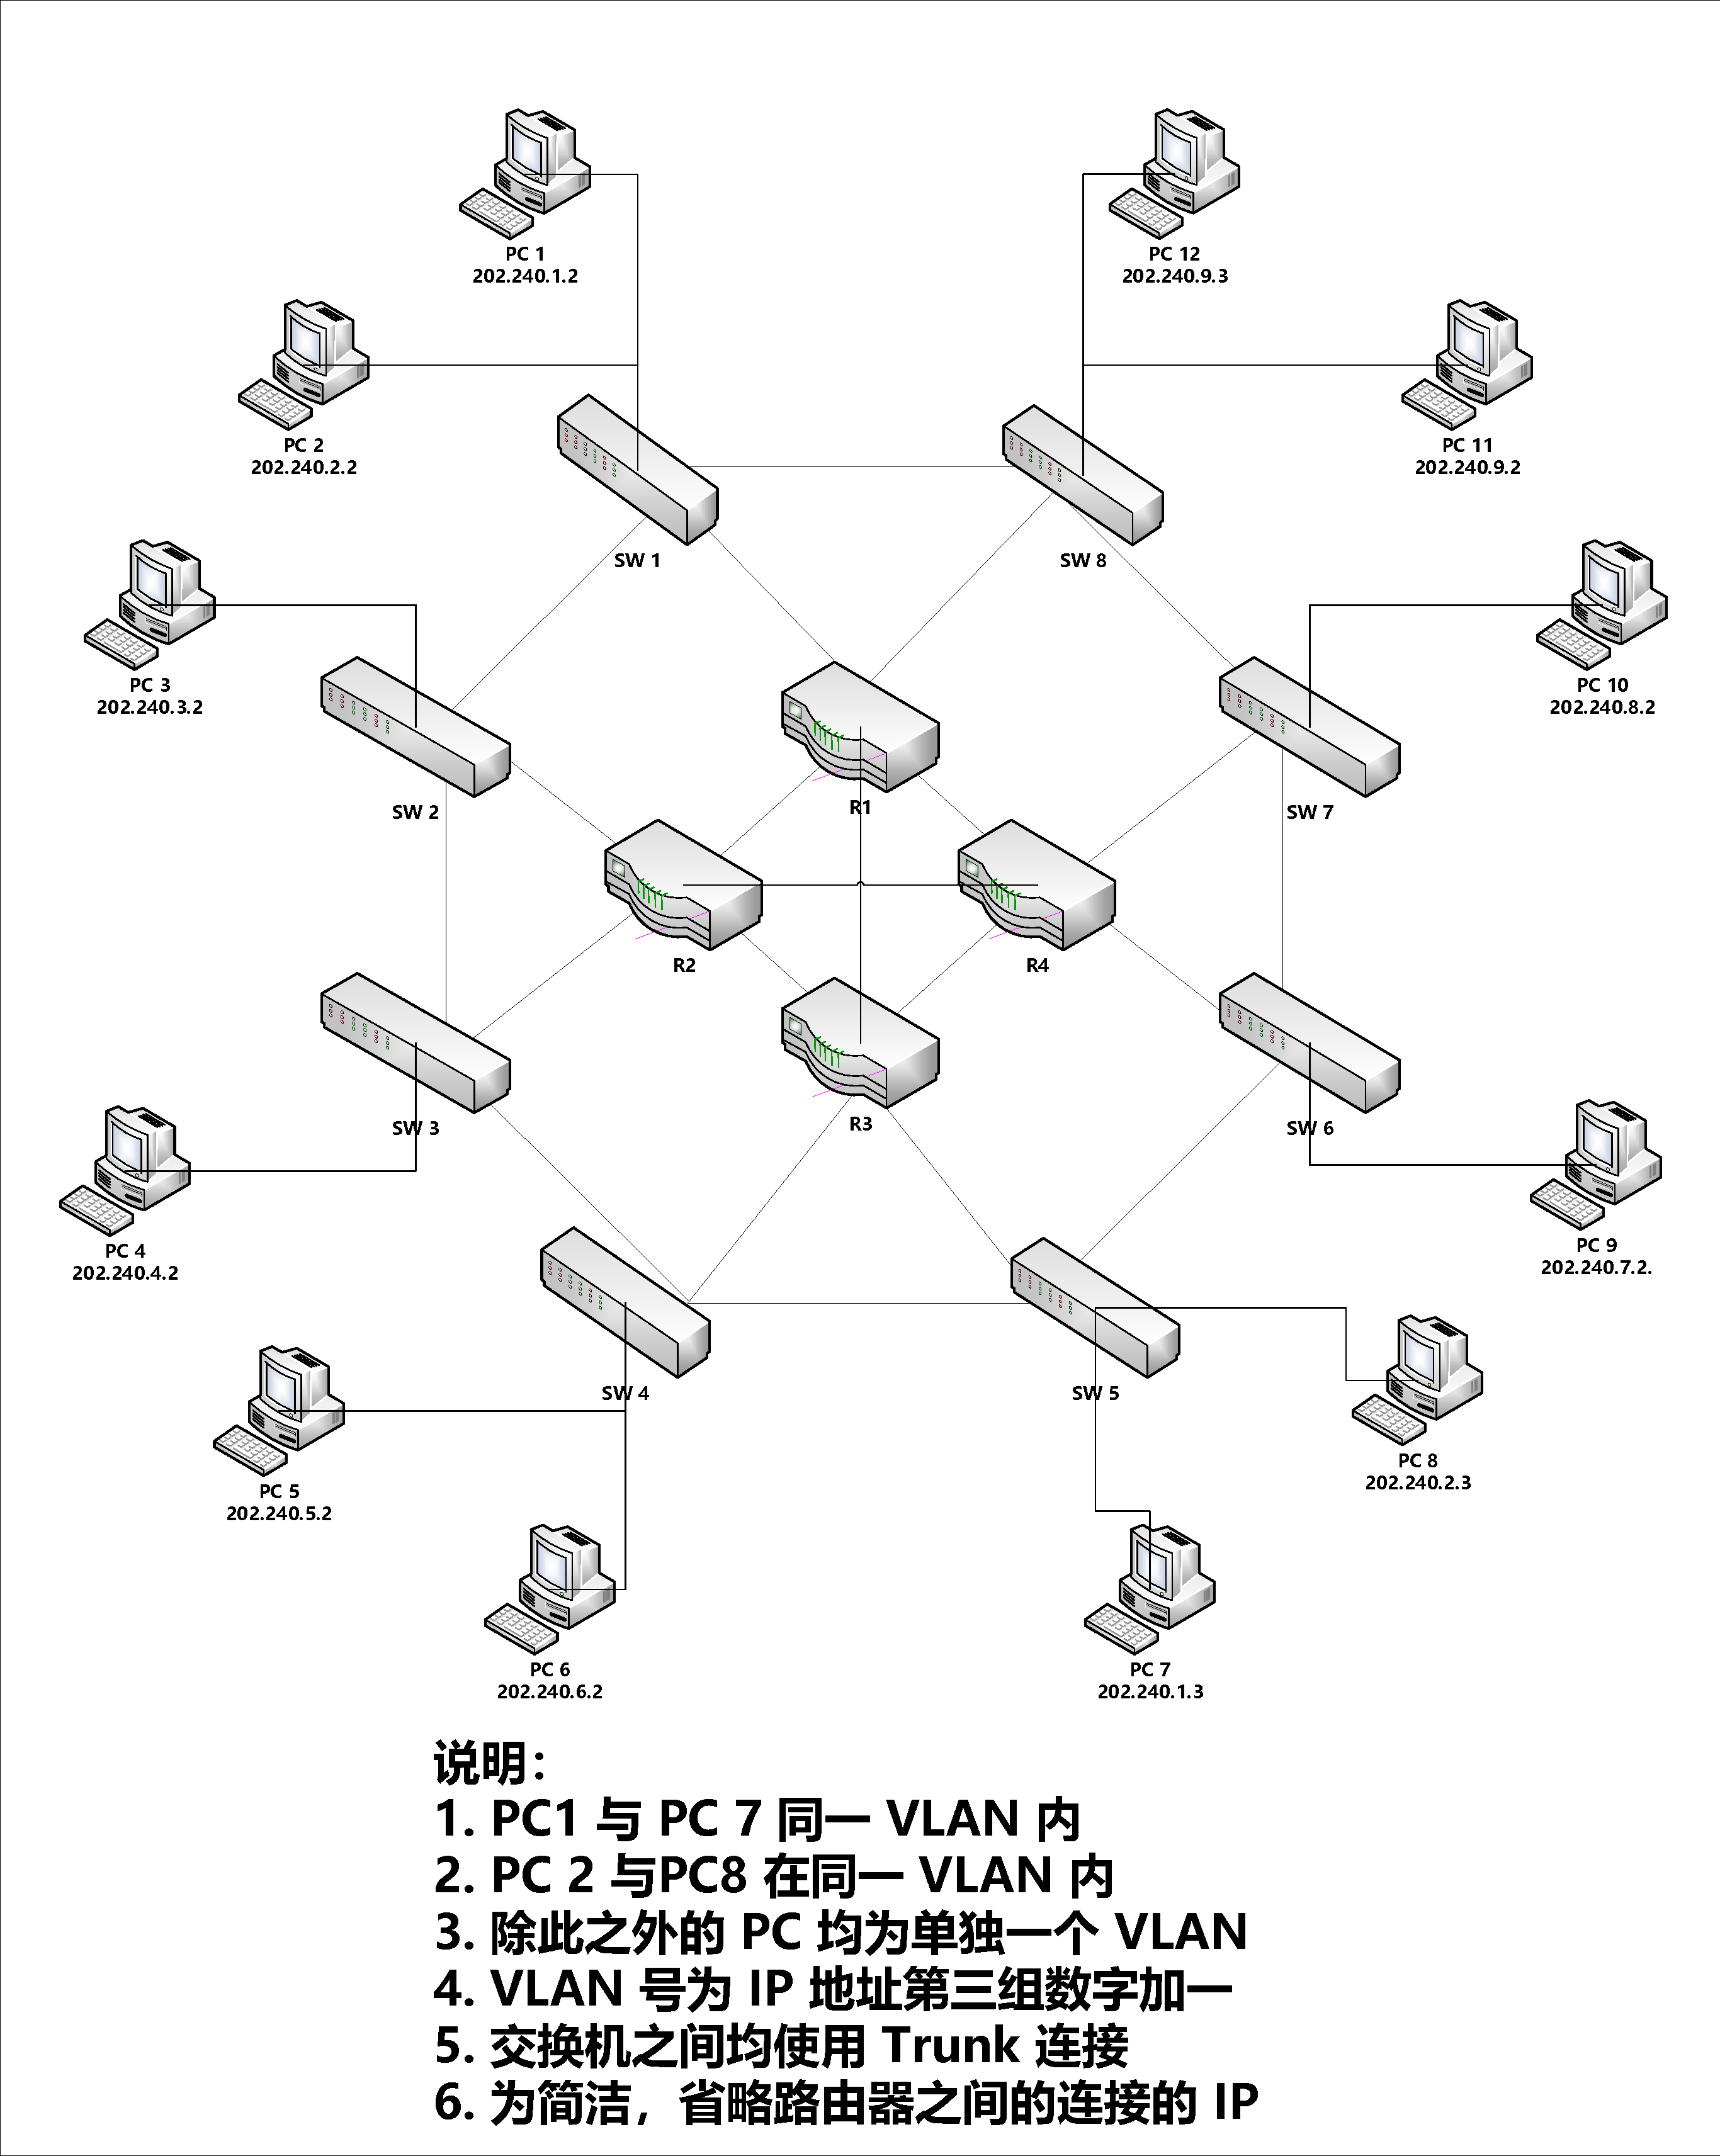
\includegraphics[width=0.94\textwidth]{top}

因为设备过多,放出其全部配置流程比较占用空间,因此我们在此只选择几个典型设备展示其配置流程。

对于 PC,其配置流程很简单,只需要为端口指定 IP,如下是在 \textbf{PC1} 上进行配置的流程:
\begin{lstlisting}
Router>en
Router#conf
Configuring from terminal, memory, or network [terminal]?
Enter configuration commands, one per line.  End with CNTL/Z.
Router(config)#interface f0/0
Router(config-if)#ip add 202.240.1.2 255.255.255.0
Router(config-if)#no shutdown
Router(config-if)#exit
Router(config)#
00:11:58: %LINK-3-UPDOWN: Interface FastEthernet0/0, changed state to up
00:11:59: %LINEPROTO-5-UPDOWN: Line protocol on Interface FastEthernet0/0, changed state to up
\end{lstlisting}
其余 PC 与之类似,只有 IP 地址不同。

对于路由器和交换机,我们有两种配置方式,两种方式的区别是是否将路由器交换机与路由器之间相连的口配置上 \texttt{trunk} 链接。在我们的设置中,\texttt{SW1} 以及 \texttt{SW8} 接 \texttt{R1} 的端口和 \texttt{SW4} 以及 \texttt{SW5} 接 \texttt{R3} 的端口使用 \text{trunk} 链接,其余全部使用配置相应的 VLAN 端口实现。

为了简化实现,我们的路由器之间使用 OSPF 协议进行配置。

此时 \textbf{R1} 的配置过程如下:
\begin{lstlisting}
Router>en
Router#conf
Configuring from terminal, memory, or network [terminal]?
Enter configuration commands, one per line.  End with CNTL/Z.
Router(config)#interface s 1/0
Router(config-if)#clock rate 115200
Router(config-if)#ip add 202.240.17.1 255.255.255.0
Router(config-if)#ip ospf hello-interval 5
Router(config-if)#ip ospf dead-interval 20
Router(config-if)#encapsulation PPP
Router(config-if)#no shutdown
Router(config-if)#exit
Router(config)#interface s 1/1
Router(config-if)#clock rate 115200
Router(config-if)#ip add 202.240.18.1 255.255.255.0
Router(config-if)#ip ospf hello-interval 5
Router(config-if)#ip ospf dead-interval 20
Router(config-if)#encapsulation PPP
Router(config-if)#no shutdown
Router(config-if)#exit
Router(config)#interface s 1/2
Router(config-if)#clock rate 115200
Router(config-if)#ip add 202.240.19.1 255.255.255.0
Router(config-if)#ip ospf hello-interval 5
Router(config-if)#ip ospf dead-interval 20
Router(config-if)#encapsulation PPP
Router(config-if)#no shutdown
Router(config-if)#exit
Router(config)#interface f 0/0.1
Router(config-if)#encapsulation dot1q 2
Router(config-if)#ip add 202.240.1.1 255.255.255.0
Router(config-if)#no shutdown
Router(config-if)#exit
Router(config)#interface f 0/0.2
Router(config-if)#encapsulation dot1q 3
Router(config-if)#ip add 202.240.2.1 255.255.255.0
Router(config-if)#no shutdown
Router(config-if)#exit
Router(config)#interface f 0/1
Router(config-if)#ip add 202.240.9.1 255.255.255.0
Router(config-if)#no shutdown
Router(config-if)#exit
Router(config)#no cdp run
Router(config)#router ospf 20
Router(config-router)#network 202.240.17.0 255.255.255.0 area 0
Router(config-router)#network 202.240.18.0 255.255.255.0 area 0
Router(config-router)#network 202.240.19.0 255.255.255.0 area 0
Router(config-router)#network 202.240.1.0 255.255.255.0 area 0
Router(config-router)#network 202.240.2.0 255.255.255.0 area 0
Router(config-router)#network 202.240.9.0 255.255.255.0 area 0
Router(config-router)#exit
Router(config)#exit
\end{lstlisting}
这一配置包含了两种连接方式,很有代表性。

对于交换机的连接,要做的是指定每个端口的 VLAN 号或者是否为 \texttt{trunk} 链接。例如,\textbf{SW1} 的配置方式如下:

\begin{lstlisting}
Router>en
Router#vlan database
Router(vlan)#vlan 2
VLAN 2 added:
    Name: VLAN0002
Router(vlan)#vlan 3
VLAN 3 added:
    Name: VLAN0002
Router(vlan)#vlan 4
VLAN 4 added:
    Name: VLAN0004
Router(vlan)#vlan 5
VLAN 5 added:
    Name: VLAN0005
Router(vlan)#vlan 6
VLAN 6 added:
    Name: VLAN0006
Router(vlan)#vlan 7
VLAN 7 added:
    Name: VLAN0007
Router(vlan)#vlan 8
VLAN 8 added:
    Name: VLAN0008
Router(vlan)#vlan 9
VLAN 9 added:
    Name: VLAN0009
Router(vlan)#vlan 10
VLAN 10 added:
    Name: VLAN0010
Router(vlan)#exit
APPLY completed.
Exiting....
Router#conf
Configuring from terminal, memory, or network [terminal]?
Enter configuration commands, one per line.  End with CNTL/Z.
Router(config)#interface vlan 2
Router(config-if)#exit
Router(config)#interface vlan 3
Router(config-if)#exit
Router(config)#interface vlan 4
Router(config-if)#exit
Router(config)#interface vlan 5
Router(config-if)#exit
Router(config)#interface vlan 6
Router(config-if)#exit
Router(config)#interface vlan 7
Router(config-if)#exit
Router(config)#interface vlan 8
Router(config-if)#exit
Router(config)#interface vlan 9
Router(config-if)#exit
Router(config)#interface vlan 10
Router(config-if)#exit
Router(config)#interface f1/11
Router(config-if)#switchport access vlan 2
Router(config-if)#exit
Router(config)#interface f1/12
Router(config-if)#switchport access vlan 3
Router(config-if)#exit
Router(config)#interface f1/8
Router(config-if)#switchport mode Trunk
Router(config-if)#
*Mar  1 00:56:51.242: %DTP-5-TRUNKPORTON: Port Fa1/8 has become dot1q trunk
Router(config-if)#switchport trunk allowed vlan all
Router(config-if)#exit
Router(config)#interface f1/9
Router(config-if)#switchport mode Trunk
Router(config-if)#
*Mar  1 00:56:51.992: %DTP-5-TRUNKPORTON: Port Fa1/9 has become dot1q trunk
Router(config-if)#switchport trunk allowed vlan all
Router(config-if)#exit
Router(config)#interface f1/1
Router(config-if)#switchport mode Trunk
Router(config-if)#
*Mar  1 00:56:52.433: %DTP-5-TRUNKPORTON: Port Fa1/1 has become dot1q trunk
Router(config-if)#switchport trunk allowed vlan all
Router(config-if)#exit
\end{lstlisting}

如此配置全部设备,之后我们让 \textbf{PC1} 和 \textbf{PC9} 上互相 \textbf{ping} 对方,结果如下.

\textbf{PC1} 对 \textbf{PC9}:

\begin{lstlisting}
Router#ping 202.240.7.2

Type escape sequence to abort.
Sending 5, 100-byte ICMP Echos to 202.240.7.2, timeout is 2 seconds:
...!!
Success rate is 60 percent (3/5), round-trip min/avg/max = 30/42/57 ms
Router#ping 202.240.7.2

Type escape sequence to abort.
Sending 5, 100-byte ICMP Echos to 202.240.7.2, timeout is 2 seconds:
!!!!!
Success rate is 100 percent (5/5), round-trip min/avg/max = 22/50/78 ms
\end{lstlisting}

\textbf{PC9} 对 \textbf{PC1}:
\begin{lstlisting}
Router#ping 202.240.1.2

Type escape sequence to abort.
Sending 5, 100-byte ICMP Echos to 202.240.1.2, timeout is 2 seconds:
!!!!!
Success rate is 100 percent (5/5), round-trip min/avg/max = 30/52/77 ms
\end{lstlisting}

两台机器之间可以互相 \texttt{ping} 通,说明 VLAN 配置一切正常。

\section{实验中的问题及心得}

和上一次实验一样,dynamips 的崩溃次数依然没有让我失望。最后我不得不仅仅在有必要打开虚拟设备时在打开,并尽量快速停掉没有用的虚拟机器以减小崩溃的概率。就是在这样的情况下,我最终能正常完成实验也是在付出了极多的课后时间以至于老天开眼给了我一次仅有的机会尽快地完成实验。我相信这个实验几乎是无法复现的,只有在没有验收的情况下我才敢尝试如此巨大的一张拓扑图。

至于心得,就是遇到什么困难也不要怕,微笑着面对它,消除困难的最好办法就是面对困难,坚持就是胜利。

\section{实验思考}
\subsection{如何在同一个局域网中,配置两个IP网段}
将两个 IP 网段配置为两个 VLAN,之后使用上文提到的两个方法对 VLAN 进行互连,共两种配置方法。

\subsection{选择两个不同vlan中的PC机,中间要经过trunk链路连接的路由器,阐述互相ping时的完整传输流程。}
在这里我们只保留 \textbf{SW1, SW2, R2, SW3, PC4} 这一路径后我们开始进行实验。此时包在进入 \texttt{SW1} 后经由 \texttt{SW1 - SW2} 间的 \textbf{trunk} 链接,之后进入 \textbf{R2},最后由 \textbf{R2} 发往 \texttt{SW3} 最后进入 \textbf{PC4}。

这个包在进入 \textbf{SW1} 时候被上 VLAN 2 的 TAG,在进入 \textbf{R2} 时 TAG 被剥离,进入 \textbf{SW3} 时打上了 VLAN 5 的 TAG,并在进入 \texttt{PC4} 时消失。

\subsection{一个vlan中是否可以配置两个IP网络?两个vlan是否可以配置同一个IP网络?为什么?}

都可以,实际上 VLAN 这个概念中的 V 就代表其是一个逻辑上的东西,和物理设备关系不大。两个 VLAN 配置同一个 IP 网络是在 PPT 上展示的例子,在此不再赘述。一个 VLAN 中可以配置两个IP网络,但如此配置不应出现在正确配置的网络里,因为不是交换机的正确用法。

\end{document}